\chapter{Architektur Übersicht}
\label{chap:Architektur-Übersicht}


\begin{figure}[H]
  \centering
  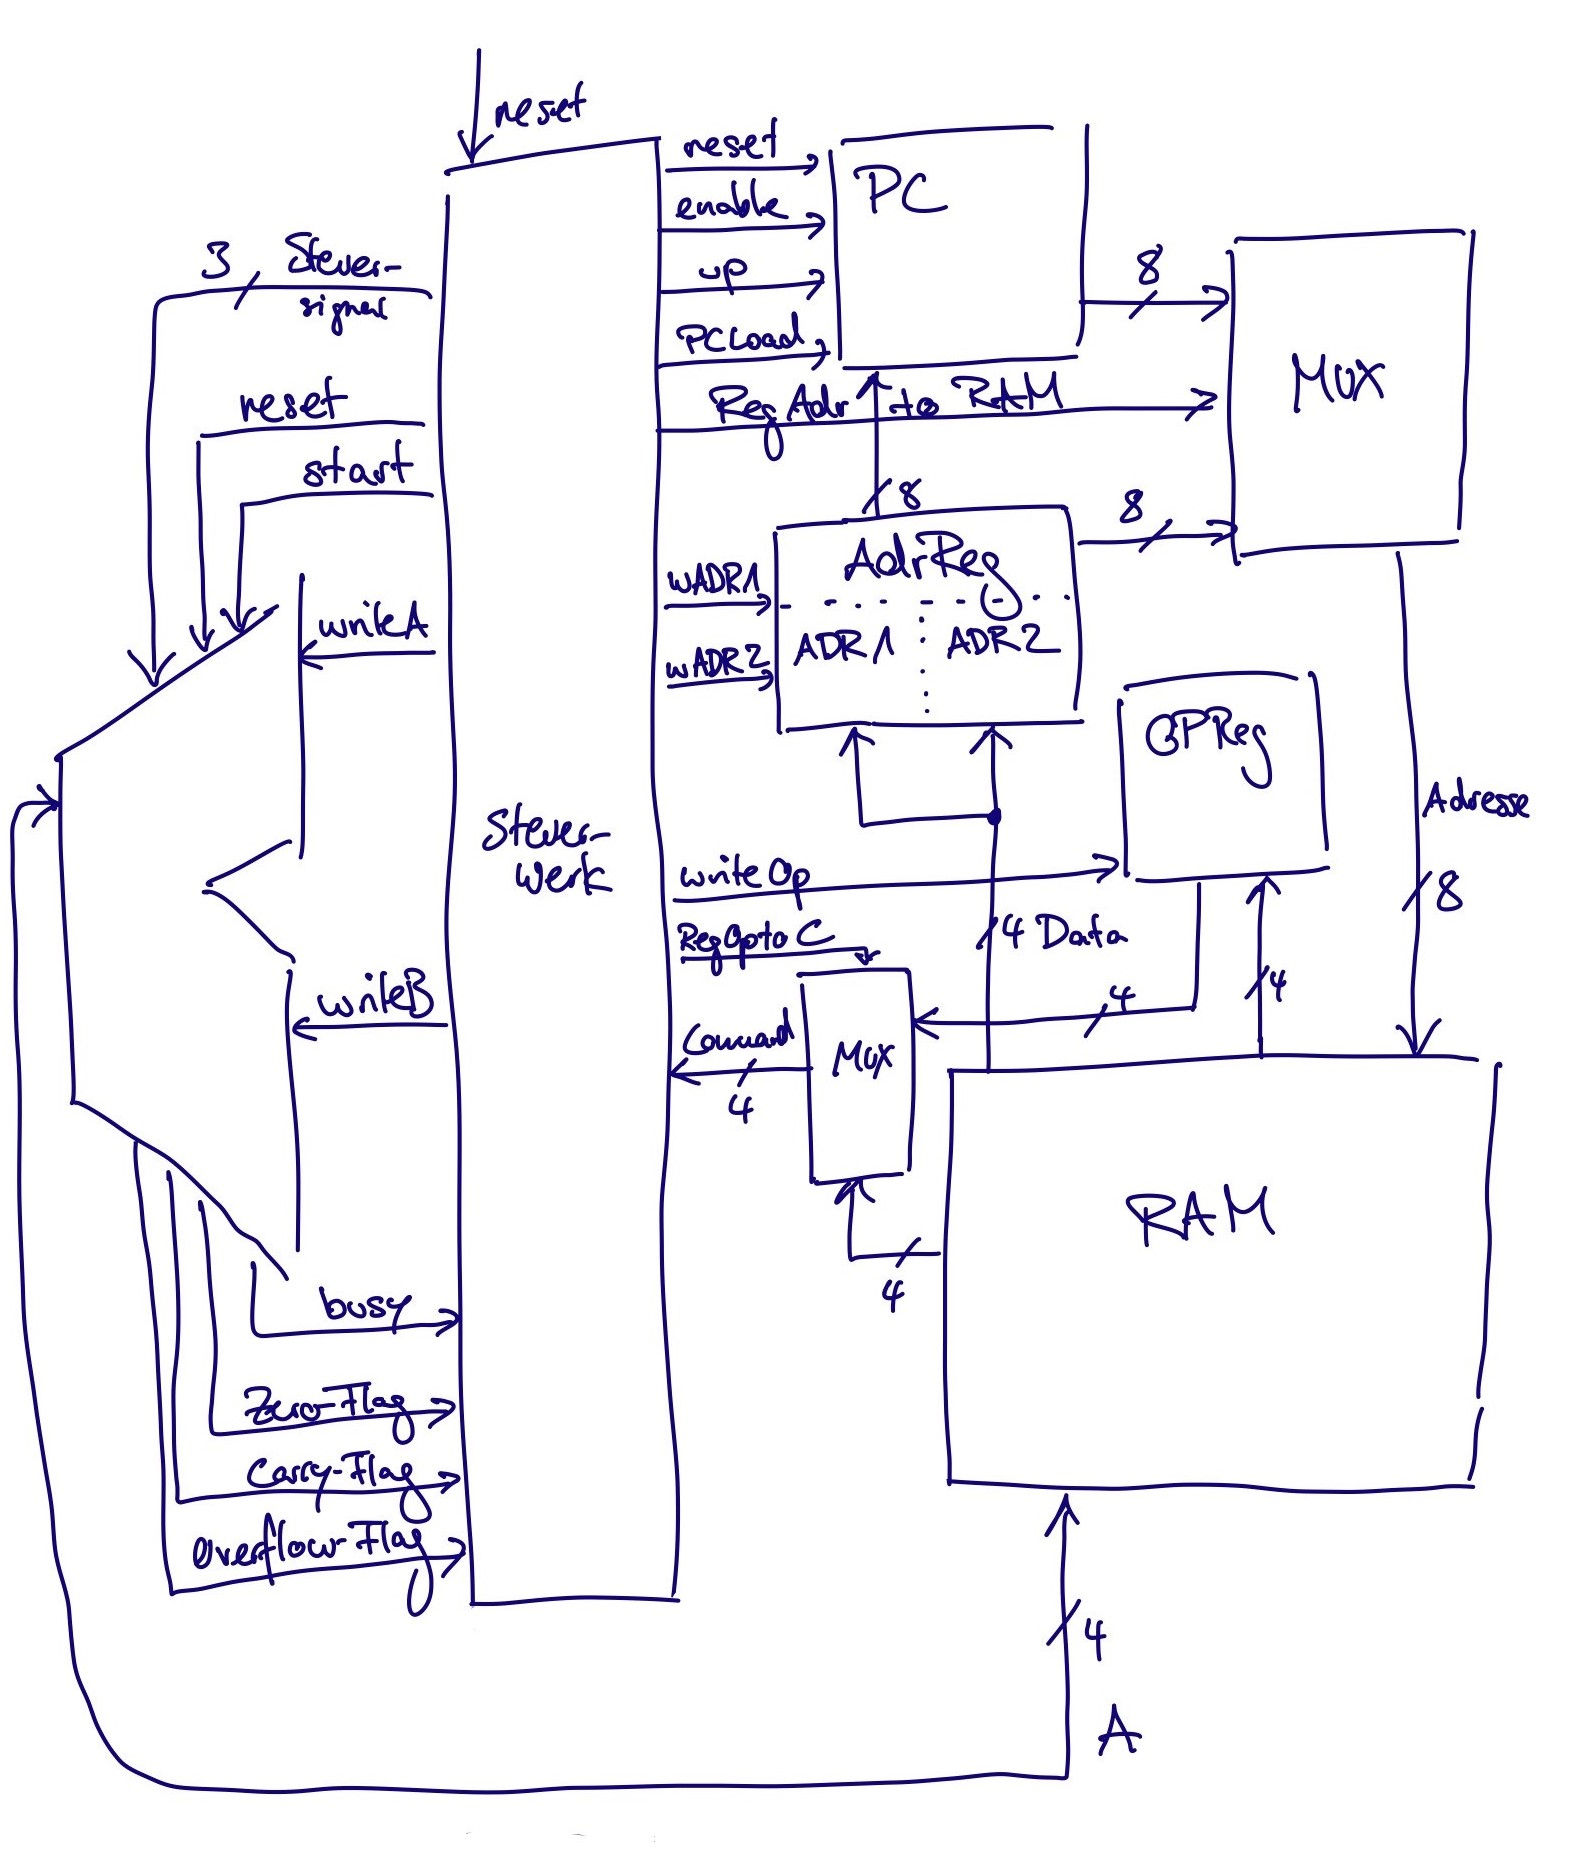
\includegraphics[scale=0.25]
  {content/figures/BSB_SW.jpg}
  \caption{First Level Blockschaltbild}
  \label{fig:blockschaltbild-first-level}
\end{figure}


\section{RAM Controller}
\label{sec:ram}

\begin{table}[H]
  \centering
  \begin{tabular}{|l|p{10cm}|}
    \hline
    \textbf{Signal} & \textbf{Beschreibung}                  \\ \hline
    \textbf{!IWE}   & Aktiviert die Schreiboperation im RAM. \\ \hline
    \textbf{IOE}    & Aktiviert die Lesefunktion im RAM.     \\ \hline
  \end{tabular}
  \caption{Signale des RAM Controllers}
\end{table}




\section{SWR}
\label{sec:SWR}

\section{Programm Counter (PC)}
\label{sec:programm-counter}

\begin{table}[H]
  \centering
  \begin{tabular}{|l|p{10cm}|}
    \hline
    \textbf{Signal}  & \textbf{Beschreibung}                                    \\ \hline
    \textbf{PC\_UP}  & Zählt den PC hoch (\texttt{1}) oder runter (\texttt{0}). \\ \hline
    \textbf{!PC\_LD} & Lädt einen neuen Wert in den PC.                         \\ \hline
    \textbf{PC\_EN}  & Aktiviert den PC für Zählvorgänge.                       \\ \hline
  \end{tabular}
  \caption{Signale des Programmzählers (PC)}
\end{table}

Der Programm Counter zählt die Adressen der Opeationen hoch, die ausgeführt werden. Dabei geht eine 8 bit Adresse in den Counter und ebenfalls wird eine 8 bit Adresse ausgegeben.


\section{Adress Register (RegADR)}
\label{sec: adress-register}

\begin{table}[H]
  \centering
  \begin{tabular}{|l|p{10cm}|}
    \hline
    \textbf{Signal}      & \textbf{Beschreibung}                               \\ \hline
    \textbf{WriteADR1}   & Schreibt die 4 MSBs der Adresse in das Register.    \\ \hline
    \textbf{WriteADR2}   & Schreibt die 4 LSBs der Adresse in das Register.    \\ \hline
    \textbf{RegADRtoRAM} & Wählt aus, ob die Adresse vom PC oder RegADR kommt. \\ \hline
  \end{tabular}
  \caption{Signale des Adressregisters (RegADR)}
\end{table}


Besteht aus zwei 2x4 Multiplexern, besteht aus zwei 2x4 Adressbits, werden für den RAM verwendet

\section{Operations Register (OpReg)}
\label{sec: operations-register}

Das Operationsregister (OpReg) speichert einen 4-Bit-Wert und verwendet dazu die Eingangssignale WriteOp und RAM3..0.

Das Signal WriteOp wird vom Steuerwerk bereitgestellt, während RAM3..0 aus dem RAM kommt. Im Fetch-Zustand ist RAM3..0 der aktuelle Befehl, während es in anderen Zuständen auch Daten oder Teile einer Adresse sein kann.

WriteOp hat die Aufgabe, die aktuell ausgeführte Operation über den Fetch-Zustand hinaus zu speichern und verfügbar zu machen. Mithilfe eines Multiplexers entscheidet WriteOp, ob ein neuer Wert aus RAM3..0 ins Register geschrieben wird oder der bereits gespeicherte Wert erhalten bleibt:

WriteOp = 0: Der aktuell gespeicherte Wert wird bei der nächsten aktiven Flanke erneut übernommen und beibehalten.
WriteOp = 1: Der Wert von RAM3..0 wird bei der nächsten aktiven Flanke in das Register geschrieben.
Diese Logik ermöglicht dem Operationsregister, bestehende Befehle über mehrere aktive Flanken hinweg zu speichern oder neue Befehle bei Bedarf aufzunehmen

















\section{ALU}

\begin{table}[h]
  \begin{tabular}{|p{1.5cm}|p{2.5cm}|p{7.4592cm}|}
    \hline
    \textbf{Pins} & \textbf{Art}  & \textbf{Beschreibung}                                    \\
    \hline
    A3..0         & Bidirektional & Register für Operand A ($A3 = MSB$)                      \\
    WriteA        & Eingang       & In A schreiben = 1 / aus A lesen = 0                     \\
    \hline
    B3..0         & Bidirektional & Register für Operand B ($B3 = MSB$)                      \\
    WriteB        & Eingang       & In B schreiben = 1 / aus B lesen = 0                     \\
    \hline
    C2..0         & Eingang       & Register für die Operation (siehe \ref{sec:Operationen}) \\
    WriteC        & Eingang       & In C schreiben = 1                                       \\
    \hline
    Start         & Eingang       & Startet die Operation (asynchron)                        \\
    \hline
    Reset         & Eingang       & Beendet die Operation (synchron)                         \\
    \hline
    CLK           & Eingang       & Clock                                                    \\
    \hline
  \end{tabular}
  \caption{Eingänge der ALU}
  \label{fig:Eingänge der ALU}
\end{table}


\begin{table}[h]
  \centering
  \begin{tabular}{|l|p{11cm}|}
    \hline
    \textbf{Pins} & \textbf{Beschreibung}                                               \\
    \hline
    BLA           &
    Gibt vorausschauend die Busy-Flag an, falls Busy mit der nächsten aktiven Flanken
    auf 0 gesetzt wird. BLA entspricht entweder Busy oder ist bereits vor der Flanke auf 0,
    nach der Busy ebenfalls auf 0 gesetzt wird.                                         \\
    \hline
    Busy          & Gibt an, ob die ALU aktuell eine Operation durchführt.
    Wenn Busy gesetzt ist, darf von außen nicht in die Register geschrieben werden.     \\
    \hline
    Carry         & Übertrag bei Addition oder Subtraktion (unsigned)                   \\
    \hline
    Overflow      & Überlauf bei Addition oder Subtraktion (signed; 2er-Kompl.)
    Das Additions- bzw. Subtraktionsergebnis ist ungültig, wenn Overflow gesetzt ist.   \\
    \hline
    Equal         & Gibt an, ob die Zahlen in Register A und B bitweise identisch sind. \\
    \hline
    Zero          & Gibt an, ob das Ergebnis der Operation an jeder Bitstelle 0 ist.    \\
    \hline
  \end{tabular}
  \caption{Ausgänge der ALU}
  \label{fig:Ausgänge der ALU}
\end{table}
